
\documentclass[pdftex,12pt,xcolor=pdftex,table]{beamer}
\synctex=1
\usepackage{comment}
\usepackage{etex}
\usepackage{amsmath}
\usepackage{amsthm}
\usepackage{amsfonts}
\usepackage{amssymb}
\usepackage{latexsym}
\usepackage{mathtools}
\usepackage[english]{babel}
\usepackage[utf8]{inputenc}
\usepackage{tikz}
\usetikzlibrary{calc,matrix,shapes,arrows}
\usepgflibrary{shapes.arrows}
\usepackage[nomessages]{fp}
\newcounter{mycols}
\usepackage{graphicx} 
\usepackage{booktabs} 
\usepackage[sort]{natbib}
\usepackage{bibentry}
\usepackage{layout}
\usepackage[justification=centering,figureposition=bottom]{caption}
\usepackage{longtable}
\usepackage{lscape}
\usepackage{rotating}
\usepackage[figtopcap,center,scriptsize]{subfigure}
\usepackage{appendix}
\usepackage{setspace}
\usepackage[multiple,stable]{footmisc}
\captionsetup[longtable]{width=.75\textwidth}
\nocite{*} 

\mode<presentation> {
\usetheme{CambridgeUS}
}

%----------------------------------------------------------------------------------------
%	TITLE PAGE
%----------------------------------------------------------------------------------------

\title[Population diversity and development]{Does Population Diversity Matter for Economic Development in the Very Long Term?  \\  Historic Migration, Diversity and County Wealth in the US
}

\author{Andrés Rodríguez-Pose \and
Viola von Berlepsch 
}
\institute[]{Economic Growth and Comparative Development Course \\  Sergio Briceño and Diana Ricciulli \\ Contact information: dc.ricciulli10@uniandes.edu.co}


\date{\today} 

\begin{document}

\begin{frame}
\titlepage 
\end{frame}

\begin{frame}
\frametitle{Overview} 
\tableofcontents 
\end{frame}

%----------------------------------------------------------------------------------------
%	PRESENTATION SLIDES
%----------------------------------------------------------------------------------------

%------------------------------------------------
\section{Motivation} 

\begin{frame}
\frametitle{Motivation}

\begin{itemize}
\item In 2015, migration stock numbers worldwide exceeded expectations and rose to 244 million (UNDESA, 2016).
\item The analysis of the economic implications of migration is of utmost importance.
\item The majority of existing studies focus on the short term economic impact of migration (Altonji and Card, 1991; Friedberg and Hunt, 1995; Bijak et al., 2007), while the medium to long-term effects have been mostly neglected.
\end{itemize}

\end{frame}

%------------------------------------------------
\section{Research question} 

\begin{frame}

\frametitle{Research question}
\begin{itemize}
\item Does having a very diverse population at one point in time lead to persistently higher levels of economic growth? Or is the economic impact of diversity only evident in the short term, vanishing once the different population groups become part of the society’s “melting pot”?
\medskip{}
\item \textbf{Hypothesis:} Time will not significantly alter the impact of diversity on economic development. We assume that a highly fragmented (highly polarized) society will maintain its positive (negative) impact consistently in the short, medium and long term.
\end{itemize}

\end{frame}

%------------------------------------------------
\section{Related literature} 

\begin{frame}
\frametitle{Related literature}
\small{
Two lines dominate the debate, each one using different measures of diversity:
\begin{block}{Diversity as growth-enhancing}
This literature uses population fractionalization measures. It is an index that assumes that the greater the number of groups, the greater the diversity assumed in a society, which positively influences the growth potential. 
\end{block}

\begin{block}{Diversity as growth-reducing}
The majority of literature in this area refers to polarization and segregation measures, which emphasize the relative size of groups and the distance that separates them. These indices aim to capture the social tension and conflict dimension linked to a heterogeneous population.
\end{block}
}

\end{frame}

%------------------------------------------------

\begin{frame}
\frametitle{Diversity as growth-enhancing}

\small{
\textbf{Thesis:} Diversity as a central engine of innovation and creativity, which in turn fosters technological growth and progress.

\begin{itemize}
\item The connection between diversity and innovation (Jacobs, 1961; 1969).
\item Qualified and liberal people prefer to live in various regions, skilled jobs and innovation will be grouped into these same areas (Florida, 2002).
\item The speed of technological progress driven by the incoming population does not depend on the size of the influx, but on its composition (Bove and Elia, 2017).
\end{itemize}
}


\end{frame}

%------------------------------------------------

\begin{frame}
\frametitle{Diversity as growth reducing}

\small{
\textbf{Thesis:} The presence of various groups as a destabilizing factor within a society that increases the potential for unrest and social conflict.

\begin{itemize}
\item Low school performance, financial debt, and poor quality of infrastructure are consequences of high levels of segregation (Easterly and Levine, 1997).
\item La Porta et al. (1999), Mauro (1995) and Easterly et al. (2006) find that the most fragmented societies reduce the performance of the public sector and generate poor institutions.
\end{itemize}
}


\end{frame}

%------------------------------------------------

\section{Context}

\begin{frame}
\frametitle{Context}

\begin{figure}
	\begin{center}
	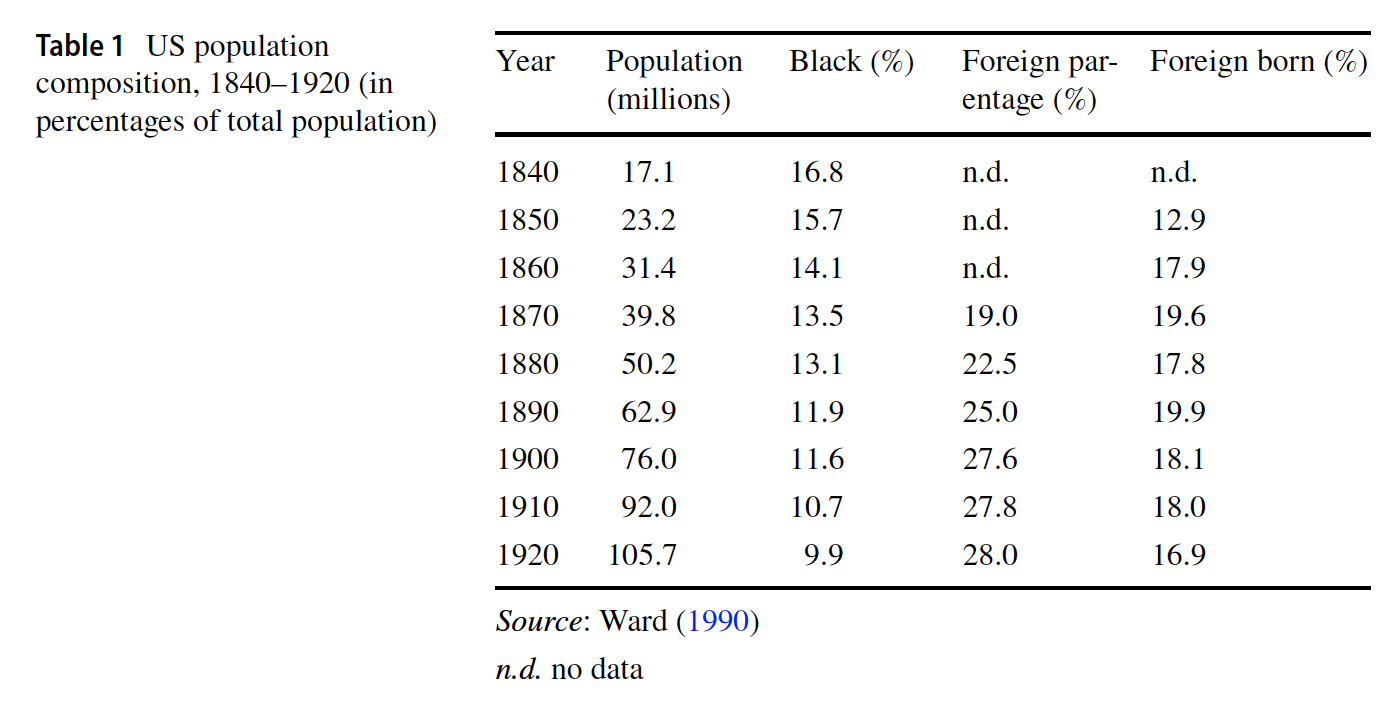
\includegraphics[scale=0.42]{context.png} 
	\end{center}
\end{figure}

\end{frame}

%------------------------------------------------

\begin{frame}
\frametitle{Context}

\begin{figure}
	\begin{center}
	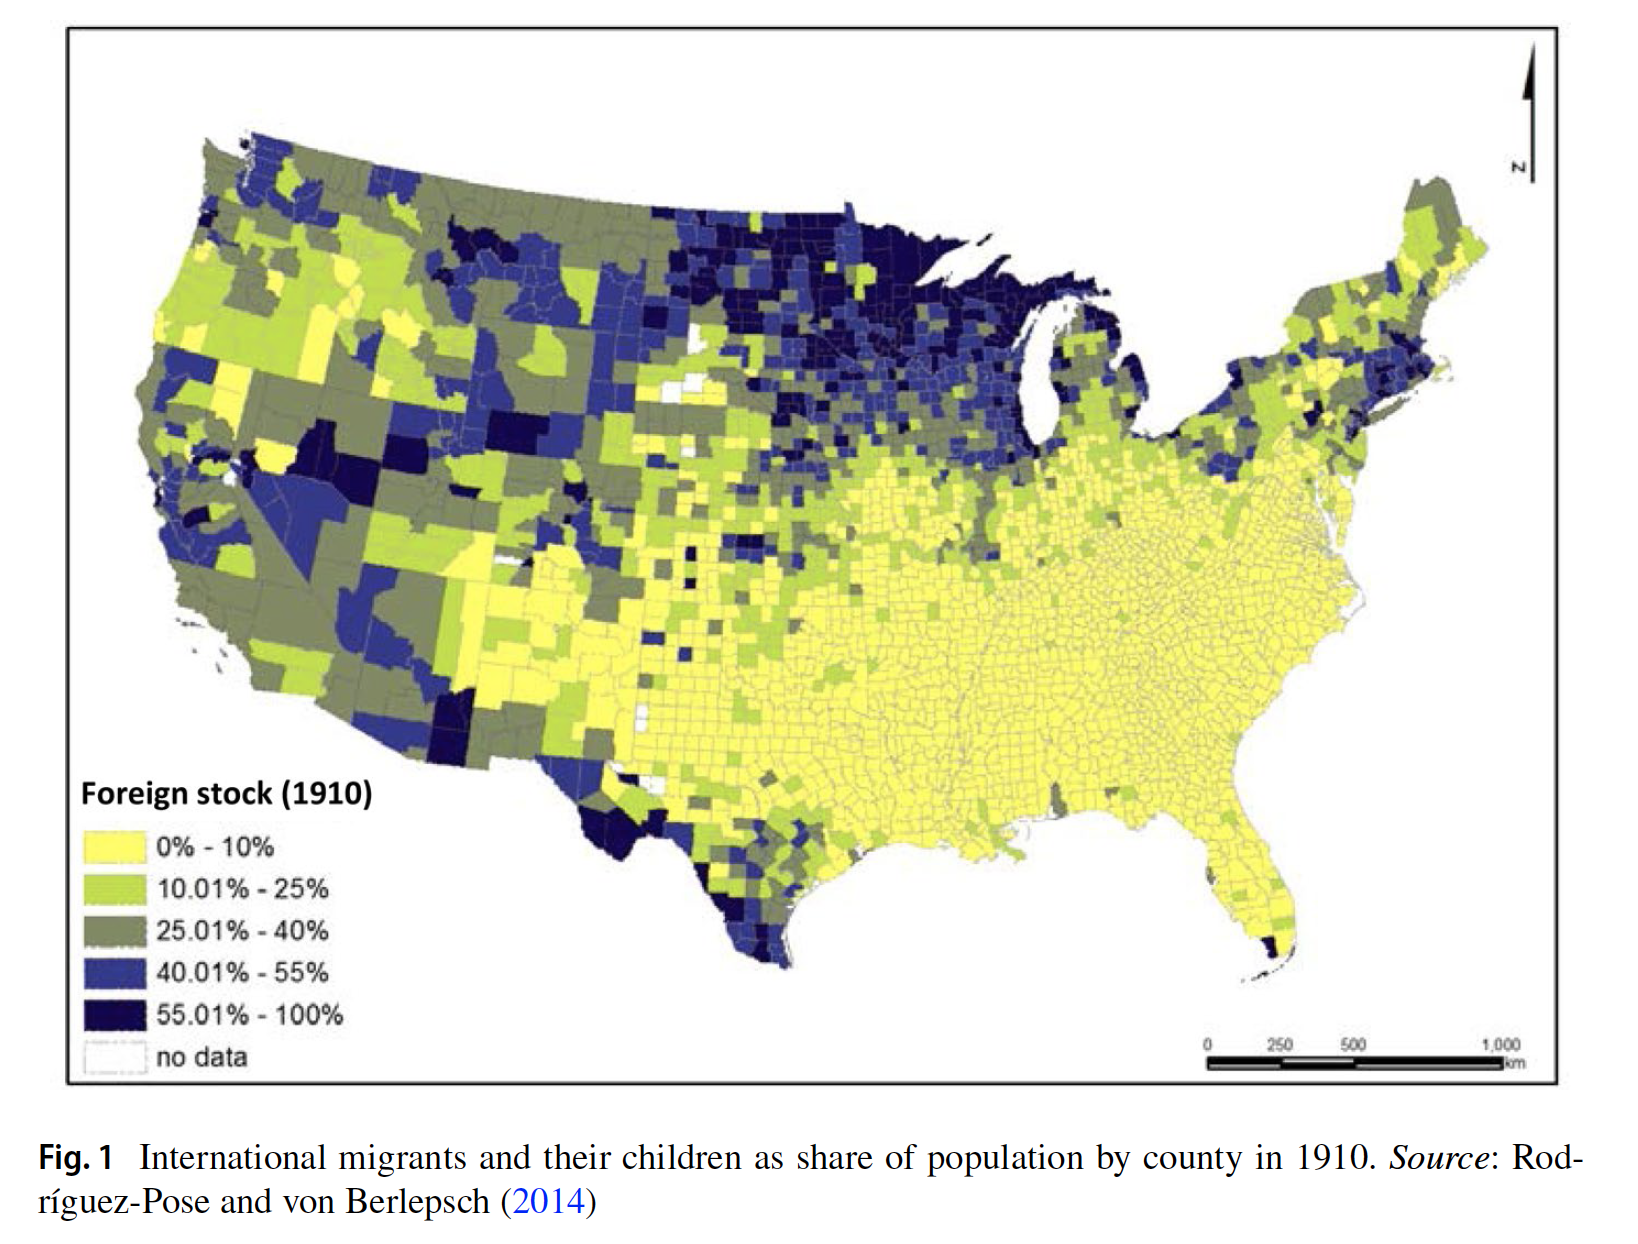
\includegraphics[scale=0.3]{context1.png} 
	\end{center}
\end{figure}

\end{frame}

%Frame_____________________________________________________________________

\section{Empirical approach and data}

\begin{frame}
\frametitle{Empirical approach}
\framesubtitle{Model 1: The case of diversity}

$y_{i,t}=\alpha+\beta Fract_{i,t_{o}}+\lambda Pol_{i,t_{0}}+\partial X_{i,t-k}+\theta Z_{i,t_{0}}+\mu state+\varepsilon_{is}$

\medskip{}

\small{
$y_{i,t}$: Income per capita of county $i$ in period $t$. \\
$Fract_{i, t_{0}}$: Level of fractionalization in a given county $i$ in $t_{0}$. \\
$Pol_{i,t_{0}}$: Degree of polarization in a given county $i$ in $t_{0}$. \\
$Z_{i,t_{0}}$, $X_{i,t-k}$: Vector of factors which may have influenced the development of the county $i$ at time $t_{0}$ and $t$.

\medskip{}

$t=(2010, 2000,..1900)$ \\
$t_{0}=(1880, 1900, 1910)$
}


\end{frame}


%Frame_____________________________________________________________________

\begin{frame}
\frametitle{Empirical approach}
\framesubtitle{Model 2: The case of concentration}

$y_{i,t}=\chi+\delta Conc_{i,t_{0}}+\phi X_{i,t-k}+\eta Z_{i,t_{0}}+\vartheta state+\omega_{is}$

\medskip{}

\small{
$Conc_{i, t_{0}}$: Level of concentration within the population of any given county $i$ in $t_{0}$.
}

\medskip{}

\small{
\begin{itemize}
\item Main identification problem: reverse causality $\rightarrow$ instrumental variables approach.
\end{itemize}
}

\end{frame}


%Frame_____________________________________________________________________

\begin{frame}
\frametitle{Empirical approach}
\framesubtitle{Measures of diversity and an Index of Concentration}

\begin{block}{Fractionalization}
$Fract_{i,t_{0}}=1-\sum_{g=1}^{n}s_{g,i,t_{0}}^{2}$
\end{block}

\begin{block}{Polarization}
$Pol_{i,t_{0}}=1-\sum_{g=1}^{n}\left(\frac{0.5-s_{g,i,t_{0}}}{0.5}\right)^{2}*s_{g,i,t_{0}}$
\end{block}

\begin{block}{Concentration}
$Conc_{i,t_{0}}=max\left(s_{g,i,t_{0}}\right)$
\end{block}

\end{frame}

%Frame_____________________________________________________________________

\begin{frame}
\frametitle{Data}

\small{
\begin{block}{Income per capita data}
\begin{itemize}
\item US Bureau of Economic Analysis (BEA) database
\item Current Population Survey tables (CPS) of the US Bureau of Labor Statistics (BLS)
\end{itemize}
\end{block}

\begin{block}{Fractionalization, polarization and concentration measures}
\begin{itemize}
\item Birthplace data at county level of the years 1880, 1900 and 1910, extracted from the IPUMS USA database.
\end{itemize}
\end{block}
}

\end{frame}

%Frame_____________________________________________________________________

\begin{frame}
\frametitle{Data}
\framesubtitle{Measures of diversity and an Index of Concentration}

\begin{figure}
	\begin{center}
	 \caption{\textmd{Fractionalization and Polarization Index}}
	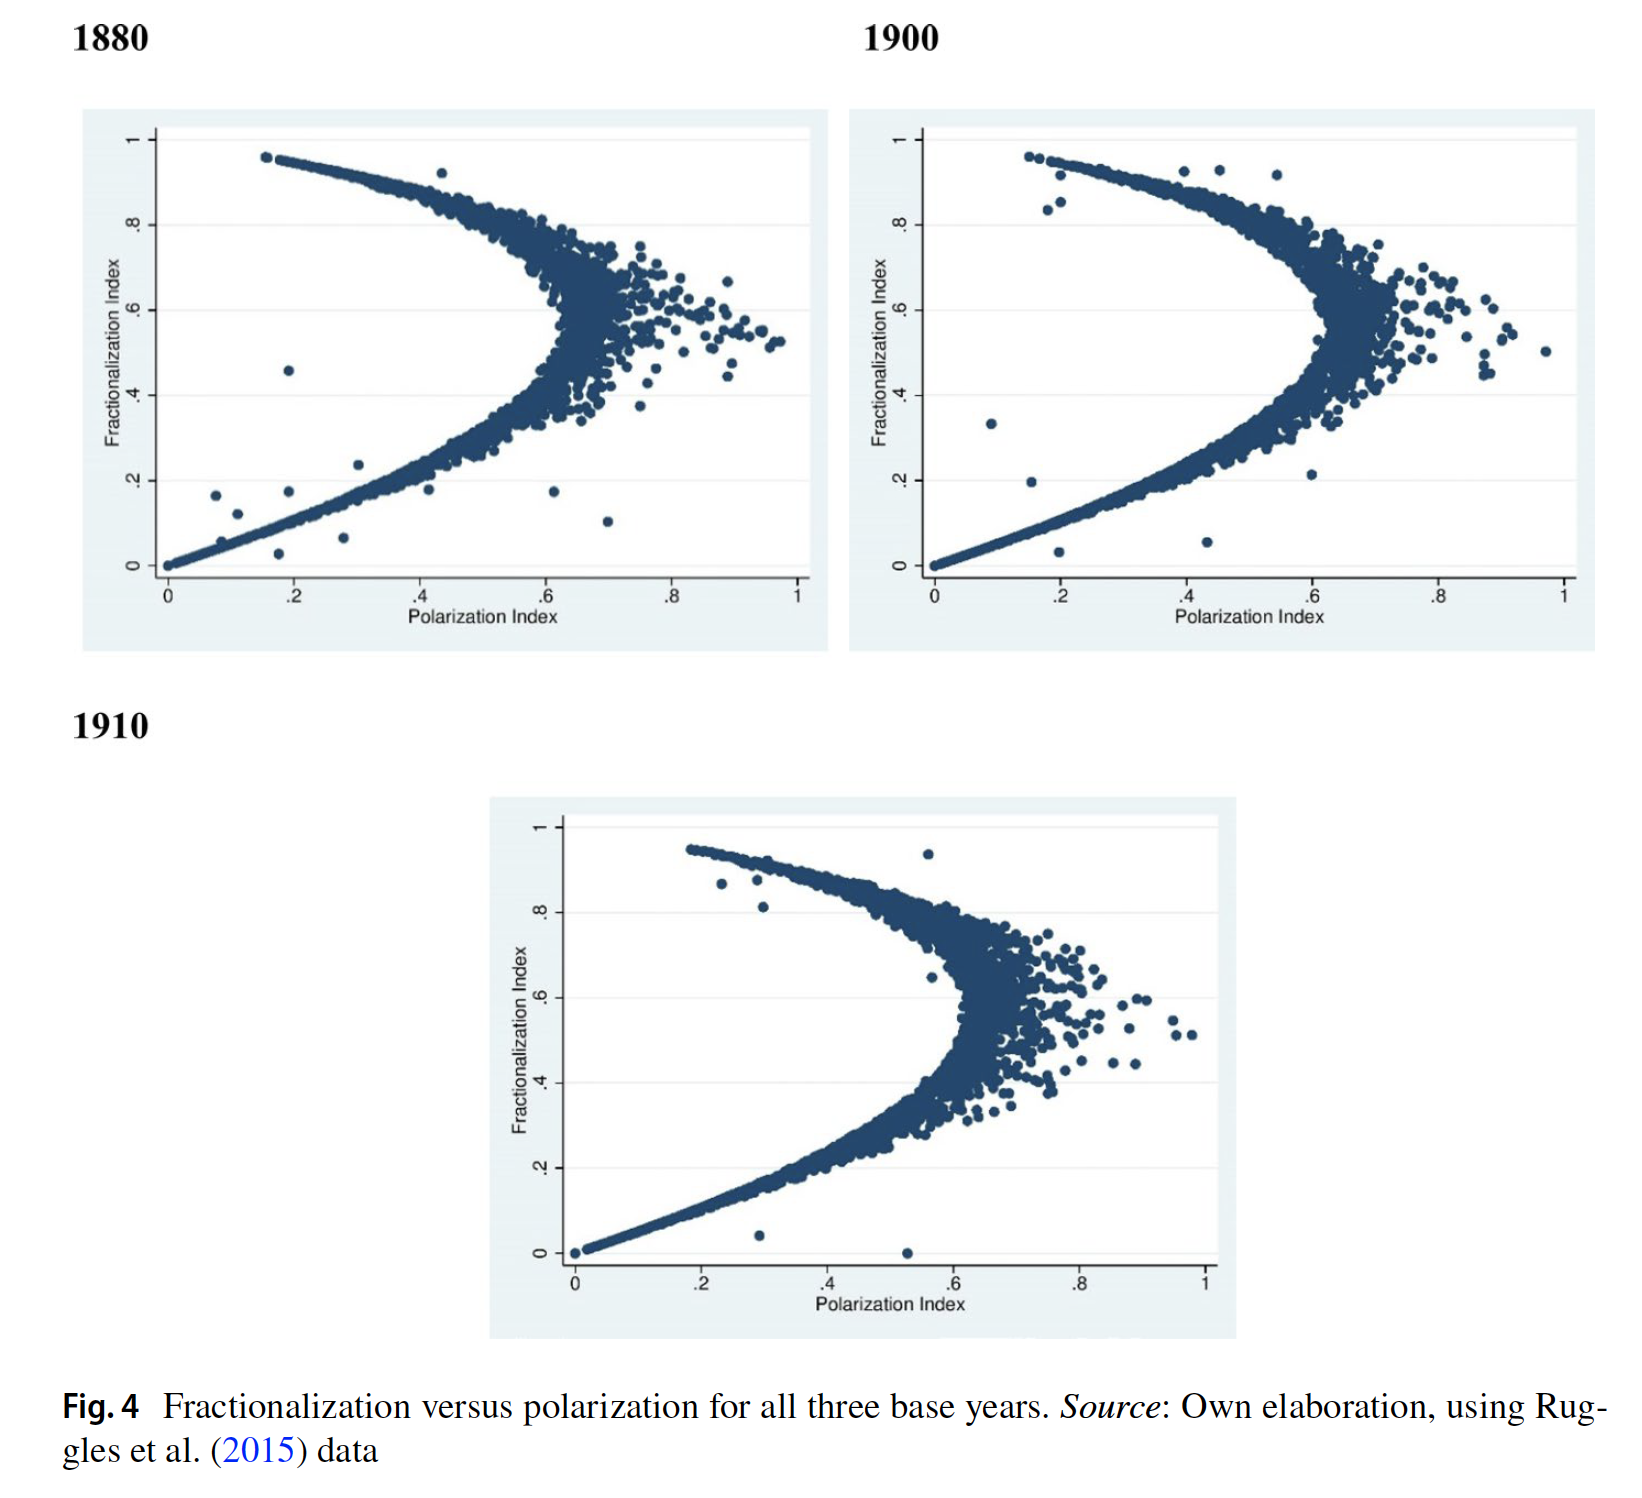
\includegraphics[scale=0.2]{measures.png} 
	\end{center}
\end{figure}

\end{frame}


%Frame_____________________________________________________________________
\section{Results}

\begin{frame}
\frametitle{Results}

\begin{figure}
	\begin{center}
	 \caption{\textmd{Results OLS diversity measures}}
	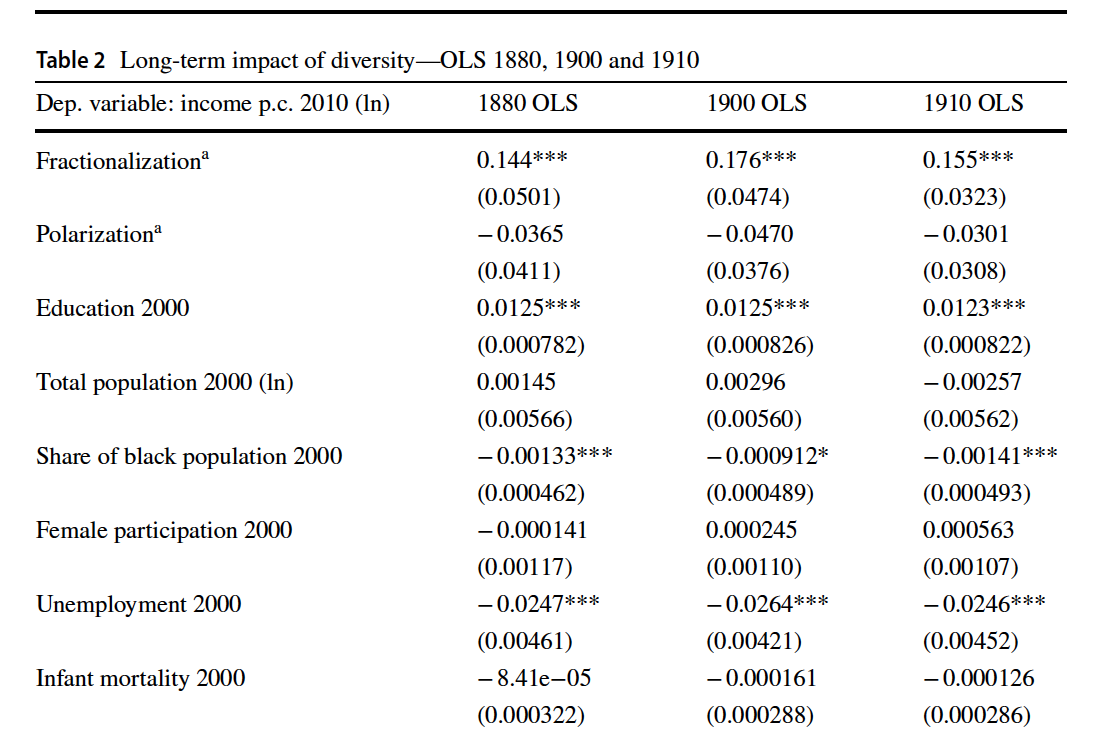
\includegraphics[scale=0.45]{results11.png} 
	\end{center}
\end{figure}


\end{frame}

%Frame_____________________________________________________________________


\begin{frame}
\frametitle{Results}

\begin{figure}
	\begin{center}
	 \caption{\textmd{Results OLS diversity measures (continued)}}
	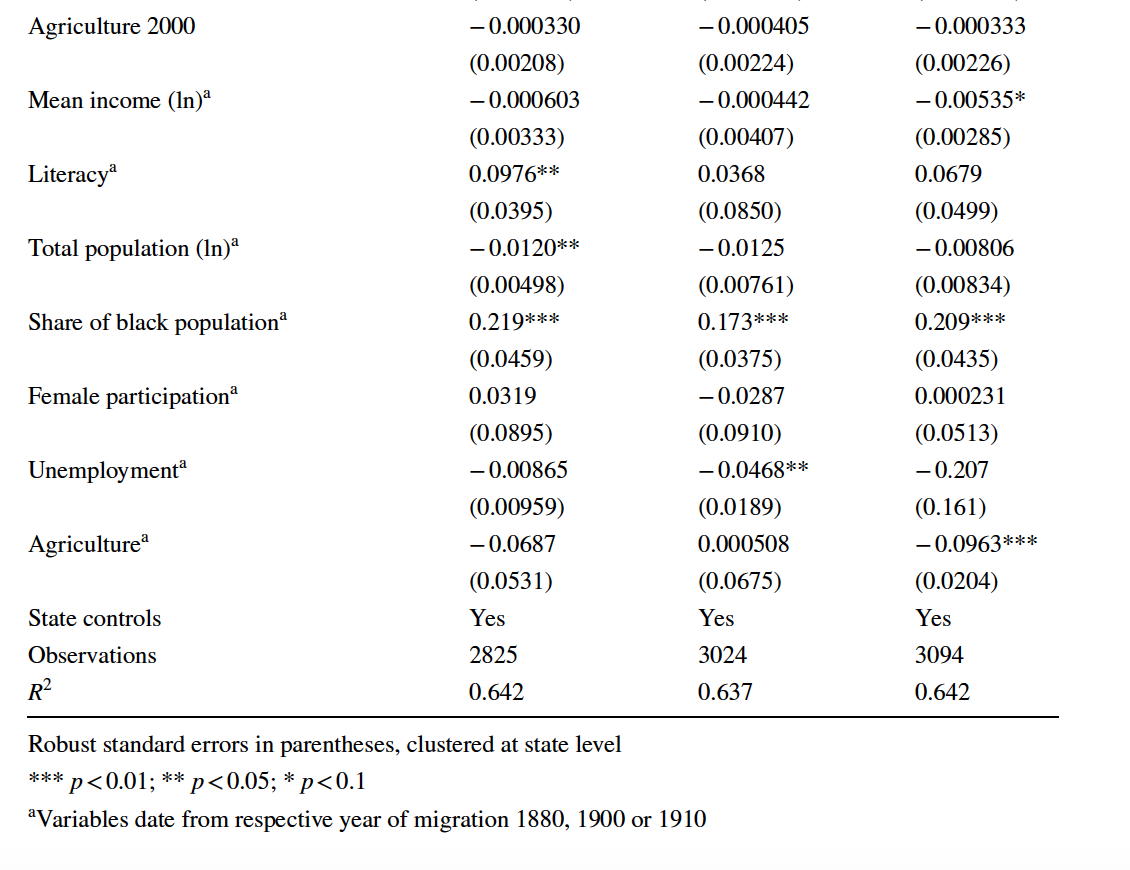
\includegraphics[scale=0.43]{results12.png} 
	\end{center}
\end{figure}


\end{frame}


%Frame_____________________________________________________________________

\begin{frame}
\frametitle{Results}

\begin{figure}
	\begin{center}
	 \caption{\textmd{Results OLS concentration measures}}
	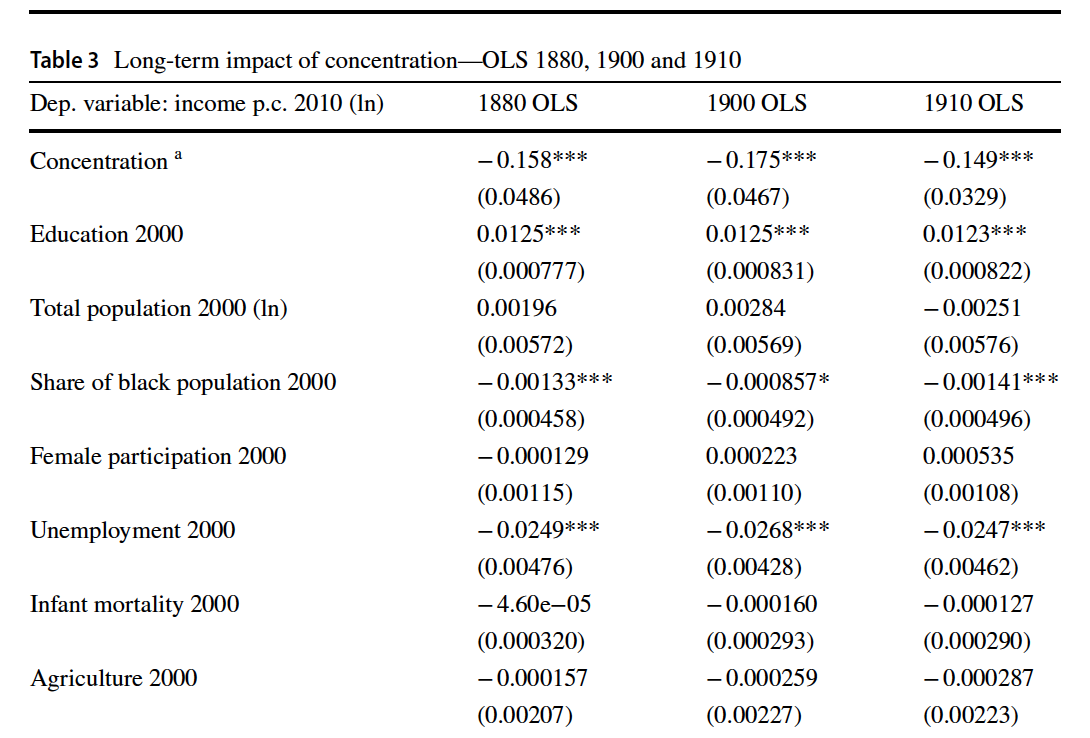
\includegraphics[scale=0.45]{results21.png} 
	\end{center}
\end{figure}


\end{frame}

%Frame_____________________________________________________________________


\begin{frame}
\frametitle{Results}

\begin{figure}
	\begin{center}
	 \caption{\textmd{Results OLS concentration measures (continued)}}
	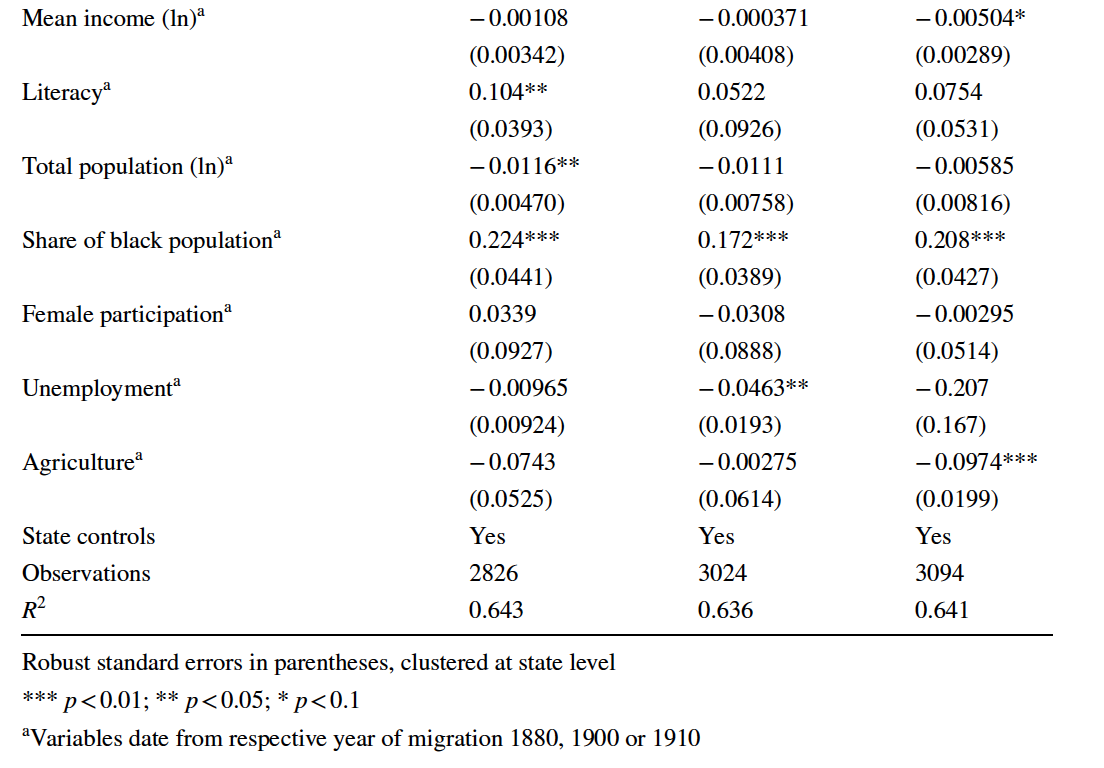
\includegraphics[scale=0.45]{results22.png} 
	\end{center}
\end{figure}


\end{frame}

%Frame_____________________________________________________________________


\begin{frame}
\frametitle{Results}

\begin{figure}
	\begin{center}
	 \caption{\textmd{IV results}}
	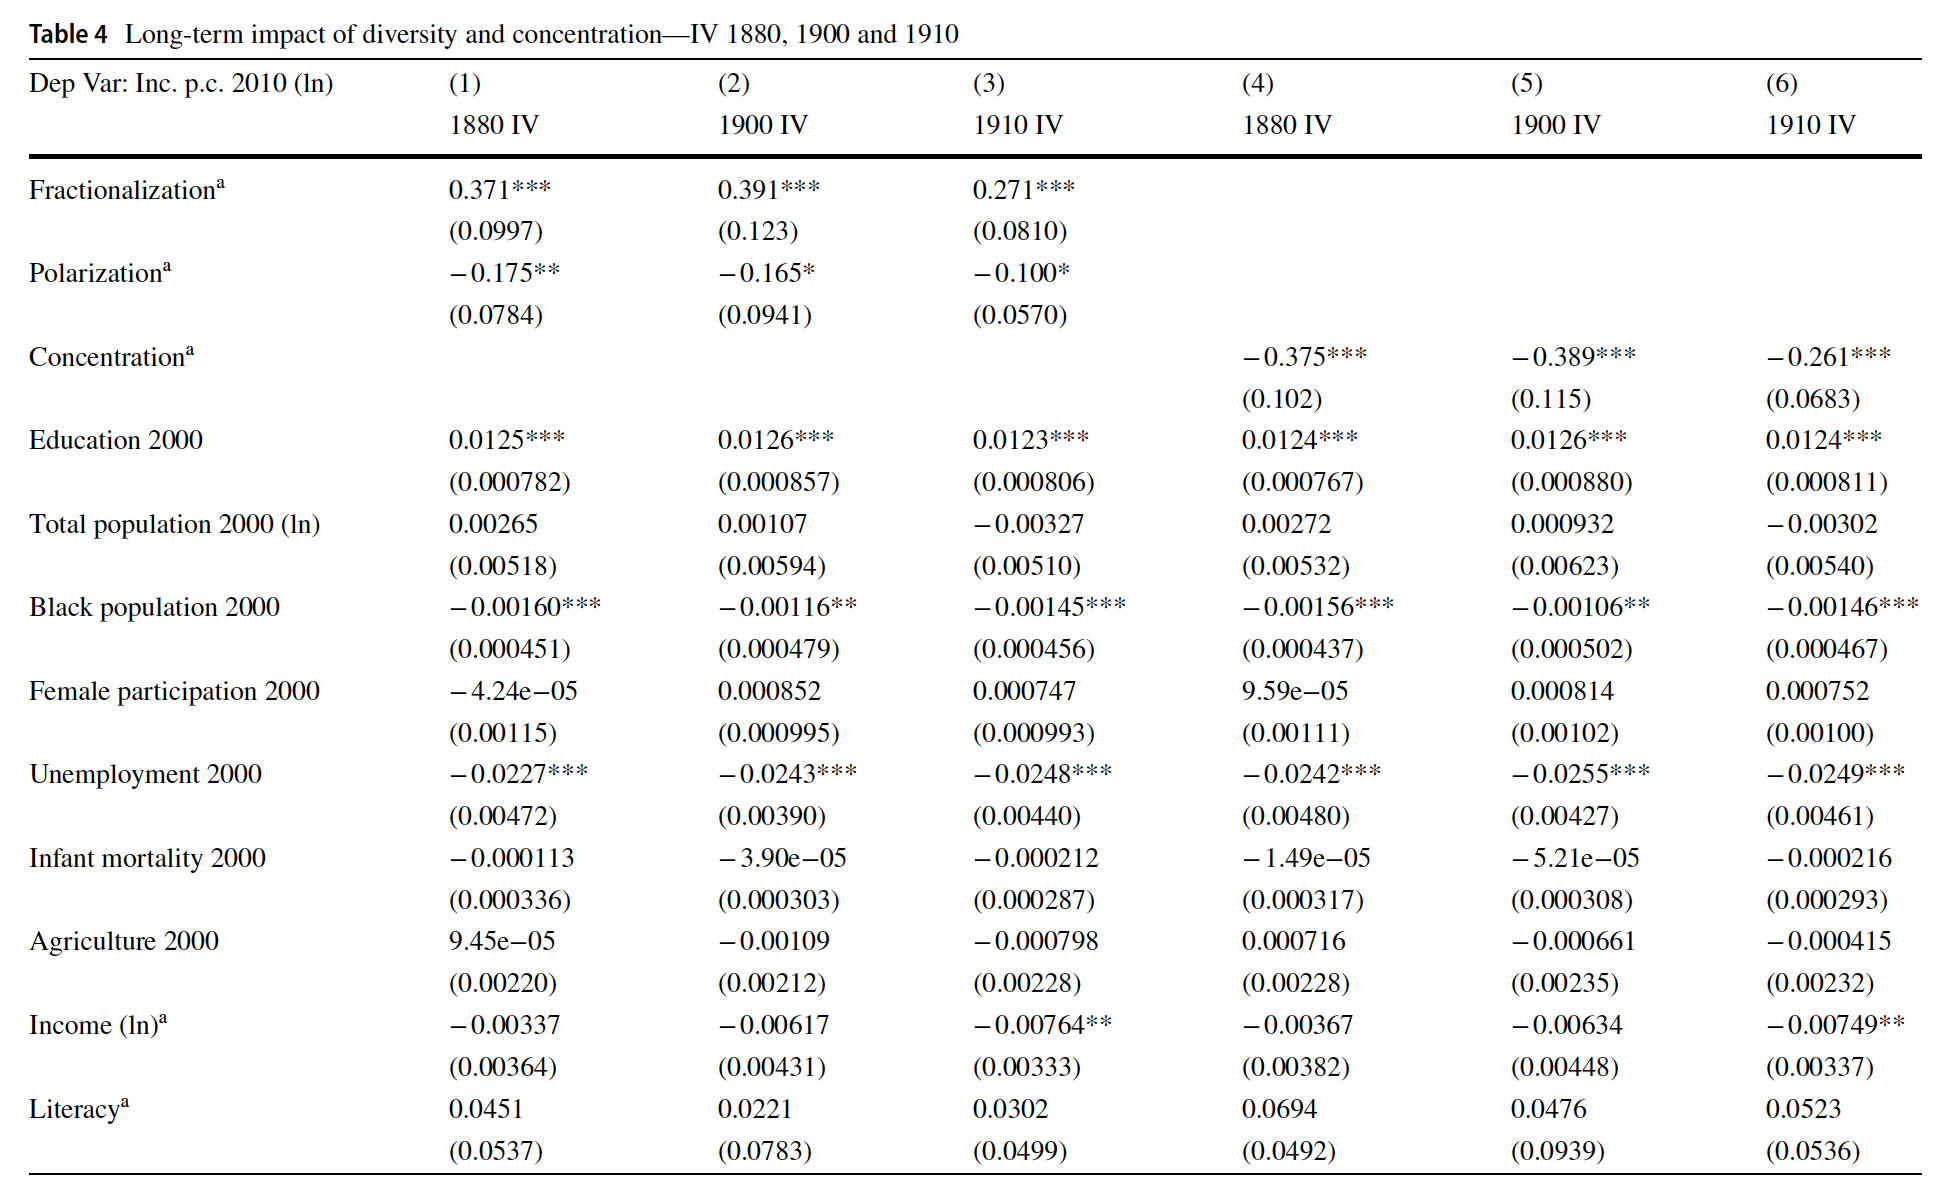
\includegraphics[scale=0.28]{robust.png} 
	\end{center}
\end{figure}


\end{frame}

%Frame_____________________________________________________________________


\begin{frame}
\frametitle{Results}

\begin{figure}
	\begin{center}
	 \caption{\textmd{Short, medium and long-term results}}
	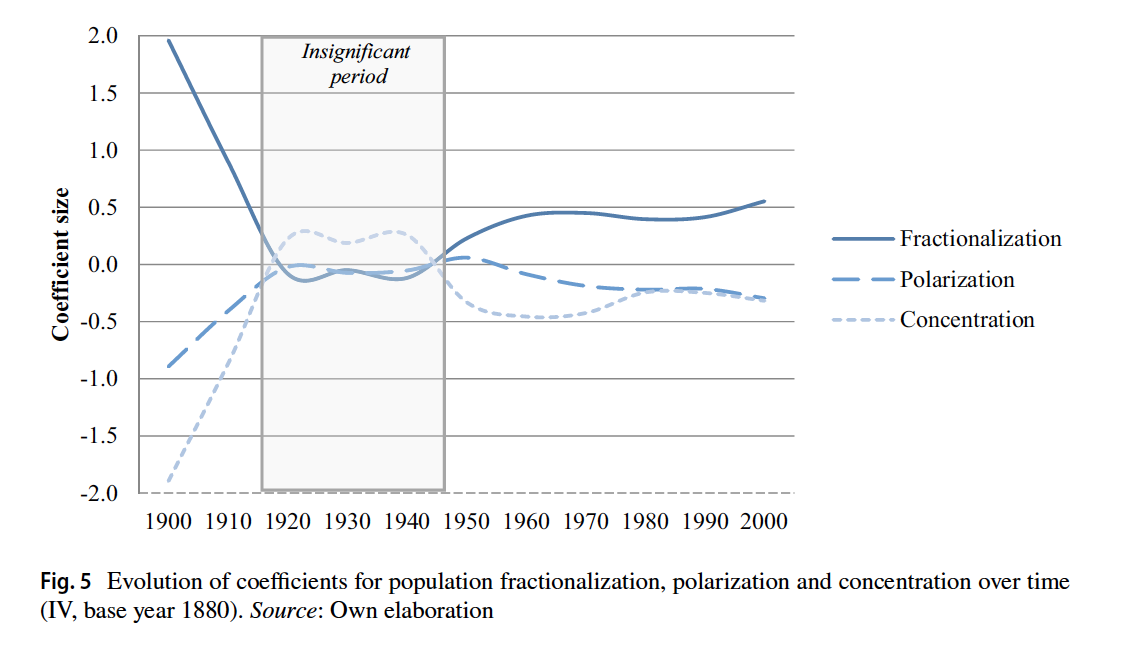
\includegraphics[scale=0.45]{results3.png} 
	\end{center}
\end{figure}


\end{frame}


%Frame_____________________________________________________________________
\section{Conclusions}

\begin{frame}
\frametitle{Conclusions}
\begin{enumerate}
\item[1.] High levels of population fractionalization have a strong and positive influence in economic development in the short, medium and long run.
\item[2.] In contrast, high levels of polarization undermine development.
\item[3.] These findings reinforce the idea that more diverse places are more innovative and productive than homogeneous places.
\item[3.] However, channels for dialogue between the different groups need to be established, as polarization in a territory appears to be detrimental for sustainable economic development. 
\end{enumerate}

\end{frame}

%Frame_____________________________________________________________________

\begin{frame}
\frametitle{References}
\footnotesize{
\begin{thebibliography}{99} 
\bibitem[Rodriguez et al., 2019]{rodriguez2019} Rodríguez-Pose, Andrés and von Berlepsch, Viola (2019)
\newblock Does population diversity matter for economic development in the very long term? Historic migration, diversity and county wealth in the US.
\newblock \emph{European Journal of Population} 35(5), 873 - 911.
\end{thebibliography}
}
\end{frame}

%----------------------------------------------------------------------------------------

\end{document} 